
\chapter{Method}
\label{chp:method}
\section{Research questions:}
\normalsize
\begin{enumerate}[label=RQ\arabic*., leftmargin=*]
    \item How can one create an algorithm to find better highlights in Counter Strike 2? \\\\
    The value of creating the proof of concept is a better highlighting algorithm than existing ones, thus making for better clips for players and spectators of the game. 
    \item What metrics are most important when developing an algorithm to find highlights in Counter-Strike 2? \\\\
    Finding out what is required for a highlight and what players prefer can help in further research into the subject and can even connect to other games where similar highlights can be of interest.
    \item How do the perceptions of what makes a good highlight differ between novice and experienced players?\\\\
    Finding out the difference between the perception of highlights of a seasoned player or someone who has not as much, or no experience gives us an insight of how one could direct highlights so that they can be enjoyed by different demographics. 
\end{enumerate}
\section{Goals:}
\normalsize
\begin{enumerate}[label=G\arabic*., leftmargin=*]
    \item Create a proof of concept of a highlight algorithm, that finds "better" highlights for a given player in a match in Counter-Strike 2.
    \item Find out what is required for an alternative highlight algorithm, what metrics players prefer
    \item Find what makes a highlight "better" and increases enjoyment when watching a highlight for players of different familiarity of Counter-Strike 2.

\end{enumerate}
Research question number 1 is connected to goal 1. Question 2 is connected to goal 2. Question 3 is connected to goal 3.\\\\
The value of these goals can affect and be used by players of Counter-Strike 2, others who are interested in the topic of highlight making/analyzing, and for spectators of the game.\\\\

\section{Research method}
We use a proof of concept and mixed-methods approach with surveys and interviews in this study. The interviews are conducted to get a better insight into what and how to weigh different metrics that will be used in the algorithm. The surveys serve the purpose of comparing our algorithm with Allstar's "play of the game". This way we can see if our algorithm could be considered better at finding highlights.
\subsection{Proof of concept of an algorithm}
\paragraph{Implementation}
\mbox{}\\

The analyzer step involved many lines of code, but most of it wasn't complex. It primarily consisted of reading player values each round and storing them in a Metrics class. This class contained all round-specific player metrics and included helper methods for easier data entry.

One challenging metric to implement was \gls{jumpshot}s. Prior to April 24, 2024, there was no way to directly determine if a player was airborne during a kill. However, Valve, the developer of Counter Strike 2, released an update that included this feature\cite{onTheOtherHandReleaseNotes}.

Previously, we had developed a workaround that analyzed the player's Y position over a two-second window surrounding a kill. We checked if the player's trajectory resembled an arch, starting high and then curving downward. This method was not perfect, as it could be fooled by ladders or stairs. Therefore, the new update greatly improved our accuracy.
\paragraph{Final Product}\mbox{}\\
The final product includes a web interface, simplifying the process of reviewing and analyzing metrics. This proved valuable for debugging analyzer issues and understanding how round scores were calculated. The process starts with uploading a demo file, which is then processed by a DemoAnalyzer instance to extract relevant data. This information is then displayed on a web page, showing all metrics for each player in every round. The round score for each round is automatically calculated, and the best round score, along with its metrics, is displayed. This is how we selected clips for the survey.

\paragraph{Weights}\mbox{}\\
When deciding how to use the metrics that we had the interviewees rate, we looked into ways to handle likert scale data and found a journal \cite{AltunaySerpil} by Serpil Aktas Altunay, Ayfer Ezgi Yilmaz (2023). In the journal we can read about the use of median, "The neutral means is the median or mid-point and the median is the 50\% sample distribution and it means 50\% of the participants have neutral to agree with opinions in a 5-point Likert scale. If the median is 4, it means 50\% of
participants have a positive opinion.". Based on this, we decided to use the median of each metric to prioritize them and use the weights in our algorithm.

\paragraph{Linear Metrics}\mbox{}\\
For all linear metrics that we have, we map the input to somewhere between 0–100. This way we handle cases where two metrics are of the same importance, but the value they give are orders of magnitude off each other. An example would be damage and kills through smokes. A player in a normal competitive match can only get a maximum of 5 kills through \gls{smokes}, but could get up to 500 damage. So if a player gets 2 smoke kills and 200 damage, both will output 40. We used a linear mapping function for this. The function is explained below \todo{make sure weights}

The metrics that use this method of scoring are, along with their minimum and maximum values used:
\begin{itemize}
    \item Damage dealt - (0-500)
    \item Headshots - (0-5)
    \item No-Scopes - (0-5)
    \item How long between each kill - (0-60)
    \item \Gls{jumpshot}s - (0-5)
    \item Hit ratio - (0-1)
    \item Distance - (0-3000)
\end{itemize}

The distance metric has a maximum of 3000, and that is based on the longest viable kill in Counter-Strike 2. This distance is from Pit to Goose on Dust2.


\begin{align*}
& \textbf{Function map:} \\
& \text{map}(v, v_{\text{min}}, v_{\text{max}}, t_{\text{min}}, t_{\text{max}}) = \frac{v - v_{\text{min}}}{v_{\text{max}} - v_{\text{min}}} \cdot (t_{\text{max}} - t_{\text{min}}) + t_{\text{min}} \\
& \quad \text{where:}\\
& \quad \quad v: \text{input value}\\
& \quad \quad v_{\text{min}}: \text{minimum input value}\\
& \quad \quad v_{\text{max}}: \text{maximum input value}\\
& \quad \quad t_{\text{min}}: \text{minimum target value}\\
& \quad \quad t_{\text{max}}: \text{maximum target value}\\ \\
& \textbf{Function mapToScore:} \\
& \text{mapToScore}(v, v_{\text{min}}, v_{\text{max}}) = \text{map}(v, v_{\text{min}}, v_{\text{max}}, 0, P) \\
& \quad \text{where:}\\
& \quad \quad P:  \text{represents the constant POINTS\_PER\_METRIC = 100}
\end{align*}

This function is the same used by a popular library, p5js \cite{p5jsMap}, that is used for interactive graphics among other things. We made a shorthand to write cleaner code, using the function mapToScore, which calls the map function, with the target min and max values already set to 0 and POINTS\_PER\_METRIC, which in our case is 100



\paragraph{Other metrics}\mbox{}\\
Certain metrics were incompatible with our scoring system, as they were not numbers or required additional processing. This section details those metrics, explaining why they did not fit with linear or exponential functions. Some metrics, such as death or what side the player was on, were simply assigned maximum points before the weighing process.


\paragraph{Kills}\mbox{}\\
For certain metrics, we increased the differences between lower and higher values. We achieved this by squaring the input before applying the mapToScore function. This resulted in a greater distinction between 4 and 5, compared to 2 and 3. This adjustment was applied only to kills, with a minimum value of 0 and a maximum value of 5.


\paragraph{HP left}\mbox{}\\

This uses an exponential decay function. This is because the lower the health of the player, the more stress it puts on the player. We picked 35 as the point where we should start increasing the points significantly. This is because an unarmored enemy does between 35-37 damage with a primary rifle. During the interviews, interviewees mentioned that being within one bullet of death, makes the highlight more impressive. We can now input the \acrshort{hp} of the player into the formula, and we get a value between 5 and 100.            
$$x) = 100 \cdot e^{-ax}  \qquad \text{where } a = 0.03$$
This is then mapped using the function mapToScore from before to a number between 0 and 100. After normalizing, we multiply this by the weight for the metric. 
This formula is an exponential decay function. It models the decrease in \acrshort{hp} Left Value as the input value (x) increases. The growth rate (a) controls how quickly the value decays. A higher growth rate means a faster decay. We used this to make sure that one bullet from death increases the value. If the player is even lower, more and more weapons will kill the player with one bullet. According to the interviews conducted, this increases the stress, and therefore how impressive the highlight is.

We choose 0.03 as the $a$ value since this makes the points for that metric go up around the 35 \acrshort{hp} mark, that being one shot away from death from most strong weapons.


\begin{figure}
    \centering
    \begin{tikzpicture}
\begin{axis}[
    axis lines = left,
    xlabel = $HP$,
    ylabel = {$f(x), points$},
]
\addplot [
    domain=0:100, 
    samples=100, 
    color=blue,
] {100 * exp(-0.03*x)};
\addplot[
    only marks,
    mark=*,
    nodes near coords,
    point meta=explicit symbolic,
]
coordinates {
    (35, 100 * exp(-0.03*35)) [One Shot]
};
\end{axis}
\end{tikzpicture}
    \caption{HP left scaling}
    \label{fig:hp-left}
\end{figure}

\paragraph{Weapon score}
For the weapons, we decided to score each weapon individually, this was each weapon gets a part of the max score for the metric. This is done by first dividing the total score for the metric, so for four weapons that will be 25 points. Then it uses that value as the max points for the weapon and rates it with the difficulty rating from the game, taken from the in-game buy menu. For an AK47, which has a difficulty rating of 4, the formula is as follows: $$ score = map(weaponDifficulty, 0, MWW, 0, PPW) $$ Here MWW is max weapon weight, and PPW is points per weapon.

This is done for each one of the weapons, added together, and finally multiplied with the weight of the weapons.


\paragraph{Side}
When looking at what side the player is playing on, either \acrshort{t} or \acrshort{ct}, we looked at the win rate for each side for the last 6 months\cite{hltvMapStats}. Here we saw a quite even split, but based on the map in the current competitive map pool, \acrshort{ct} has a higher win rate on the majority of the maps. Therefore, we assign \acrshort{t} and \acrshort{ct} -1 and 1, then in the weights, it has a negative value, so that the -1 for \acrshort{t} get awarded more points than \acrshort{ct}.


\paragraph{Technologies used}\mbox{}\\
Our algorithm was built using Typescript as the language of choice. This choice was made both out of familiarity and based on Typescript's fast iteration speed, enabling us to make changes faster than a language like C++ or Rust.

Counter-Strike 2 records everything that happens in a match in a \gls{demofile}. To parse this information, we used a library\cite{demoparser} that would give us events from the match, such as whenever a player dies, shoots, or when the rounds start or end. This library does not give us the data we need directly, so for that we need to parse information from the events available. So for that, we need to analyze the data from the demo, to later pass to our algorithm.
\paragraph{How it works}\mbox{}\\
The first part of the process to generate a highlight is to extract the metrics from the demo file. This is done in a file called DemoAnalyzer.ts, and this file handles reading the \gls{demofile} and transforming the data into a usable format. It does this by looking at different events and calculating the metrics.\\\\
The events from the demo that we use are:

\begin{itemize}
    \item player\_death
    \item player\_hurt
    \item round\_end
\end{itemize}
The next part is to store the metrics in the database. This is handled by a separate file `SaveDemoInfo.ts`. This file reads the data and puts it into tables in the database. The reason for making this a separate step was for readability and code quality. This splits up the code into the analyzer, which is only responsible for reading the data, and storing it in memory, and the SaveDemoInfo part, which only focuses on storing the data. 

The last part is the most important step. This is the algorithm itself. This takes in all the data from the demo file, as well as the weights we have defined from the interviews \ref{sec:interviews}. This then calculates a score from each metric between 0 and 100. This was done to make sure that each metric was valued the same before the weighing process. This is done using this mapping function from p5.js\cite{p5jsMap}


Following the mapping function's assignment of a value between 0 and 100, this value is then weighted to control the relative importance of each metric in determining highlight quality. For instance, is a kill through a wall more or less impressive than a kill from a long distance? Weights allow us to adjust the impact of each metric in making this determination.

\subsection{Survey}
\label{sec:survey}
A survey was created with our algorithm's outputted round and the \Gls{allstar} tool's "play of the game" round, where the same matches are evaluated on the same player, and the participant can choose which they prefer. Both rounds will be re-recorded so that a fair comparison can be made without editing and each clip starts a few seconds before an action such as shooting, spotting an enemy, or throwing utility is done.\\\\
\textbf{}
\textbf {Content for the survey:}
\begin{itemize}
    \item The respondent will be prompted to answer a question about how familiar they are with the game Counter-Strike 2. This will be presented in a type of Likert scale. 
    \begin{figure}[H]
        \centering
        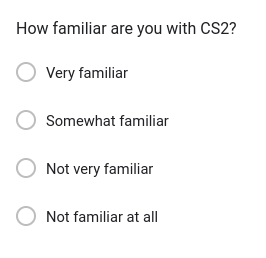
\includegraphics[width=4cm]{Images/likertscale.png}
        \caption{Likert scale}
        \label{fig:likerScale}
    \end{figure}
    \item Two clips are shown, A and B. One is the round our algorithm picked and one is the round Allstar picked, the respondent will not be told which clip is which so that there will be no biases. The respondent is then faced with the question of which clip they preferred or if the clips are indifferent. They then have the choice to write a more detailed explanation of why they picked as they did or any other input they had. There will be 18 clips in total, 9 comparisons.
    \begin{figure}[H]
        \centering
        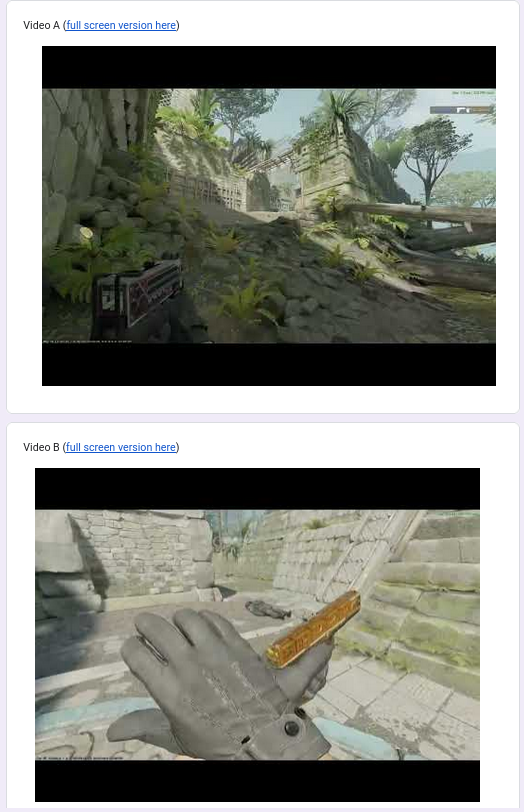
\includegraphics[width=10cm]{Images/A-B_choices.png}
        \caption{Video A and B example}
        \label{fig:VideoA_B}
    \end{figure}
    \begin{figure}[H]
        \centering
        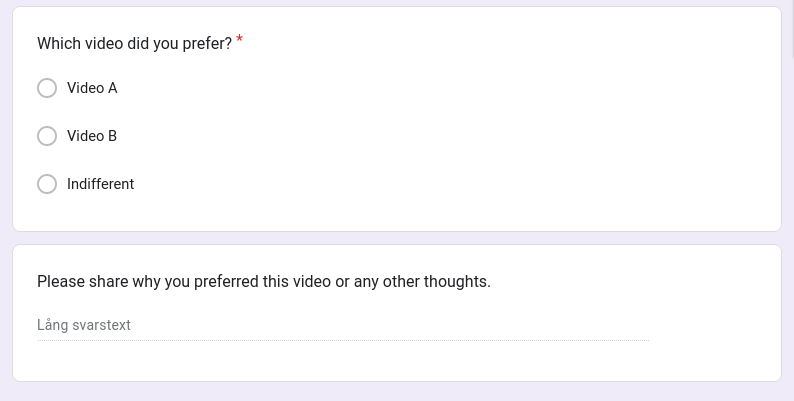
\includegraphics[width=10cm]{Images/Questions_AB_reason_Survey.png}
        \caption{Question from survey}
        \label{fig:VideoA_B_answer_reason}
    \end{figure}
\end{itemize}
The survey connects with goal 1 to see if the round from our algorithm presents is preferred over Allstar's "play of the game" round. It will also answer research question 3 by finding what people with less experience with Counter-Strike 2 think is important in a highlight.\\\\
The choice to conduct surveys was made because we want to have a large pool of opinions, as we want to see if our new algorithm is "better" than Allstar's algorithm. By choosing to do surveys, we can reach a greater amount of people. To create the surveys, we used Google Forms. The surveys were put in different forums on sites like Reddit, Discord channels and sent to people through private messages. The main targeted respondents would be those who have played Counter Strike 2, as these are the more likely to have an opinion about the clips they are shown. As we have no control of the surveys and who receives them, we put a question asking "How familiar are you with CS2?" to see the difference in opinions between people with different experience of Counter-Strike 2.\\\\
To analyze the results, we looked for the difference of what experienced and unfamiliar respondents picked to see if there are any patterns in the responses. We also analyzed if there is a clear preferred video clip from either Allstar's or our algorithm. 
\\\\

\subsection{Interviews}
\label{sec:interviews}
Interviews will be conducted before developing the algorithm to find what metrics players weigh higher, to give a better baseline on what the weights should be. \\ \\
\textbf {Interviews:}\\\\
Questions one to three in the pre interview will help us achieve the three preliminary goals and answer the research questions, as these will give us further insight into what metrics are needed and how to value them. It will also help us get a better insight to what makes a good highlight. \\\\
The choice of doing interviews was so that we could get a better understanding of how to rate different metrics and what players think is a good highlight so that we could improve our algorithm. The interviews were conducted online, where they were recorded and transcribed. The targeted respondents were people who had played Counter-Strike or similar games, with preferably different experience. To recruit these respondents, we contacted them via Discord. The respondents we interviewed were all people we knew. After the interviews were conducted, we gathered all the data we had collected and analyzed it. Things we looked for were patterns and themes that are recurring in the answers.\\\\
The answers we gathered here lay a base on how we weigh our metrics but could be used in other games that are similar to Counter-Strike 2.\\\\

\section{Validity and reliability}
Our approach of collecting data through interviews was done via \gls{Discord} where we recorded the interview. This was done so that we could have a greater reach distance wise of who we could interview. This made it possible to get a bigger size pool of different people. We also had to take into account that the people we wanted to interview had played Counter-Strike or similar games.\\\\ We recognized that it would be hard to fairly value metrics, as there a many, but the approach we took made it so that if there are metrics not mentioned by us in the interview the interviewee could have the possibility to add metrics. By picking people we had meet before, there could be issues with convenience sampling with disadvantages such as making generalization harder and bias issues. Our approach of collecting data through surveys was done via Google Forms to compare our algorithm with the existing highlight tool Allstar. The participants would not know which clip came from Allstar or our algorithm. As the clips created are from the same matches and the same persons when comparing, this makes it as unbiased as possible. The games were from our own recent matches from the dates 2024-05-09 to 
2024-05-04. In case our algorithm and Allstar outputted the same round, a new match was picked, and the instance was noted down.\\\\
The surveys were distributed to friends via Discord and Steam. We also posted the survey on gaming forums on sites such as Reddit, Twitter and Steam Discussions. By using this approach, we have no control over who answers the surveys, but we get a wide spread of people who can answer it. Problems with this approach could be the quality of data, such as unserious answers and no identity control, meaning there could be duplicates. 